\documentclass[journal]{IEEEtran}
\usepackage{graphicx}
\usepackage{amsmath}
\usepackage{amssymb} % For math symbols like \parallel, \perp
\usepackage{hyperref}
\usepackage{float}
\usepackage{subcaption} % If needed for subfigures, though likely not here
\usepackage{booktabs}
\usepackage{pgfplotstable} % To read CSV data
\usepackage{siunitx} % For units like \si{\degree}, \si{\nano\meter}
\usepackage{qrcode}

\begin{document}

\title{Investigation of Light Reflection and Polarization: Fresnel Equations - Reflection Theory}
\author{{\large IBRAHIM H.I. ABUSHAWISH} \\ % Replace with actual name
{\small Istanbul University, Dept. of Physics \\ 
Instructor: Res. Asst. Selen Nur YILMAZ \\ 
Experiment Date: 25.04.2025, Submission: \\ 
Course: PHYS2405}}

\markboth{Physics Laboratory Report, Month Year}{} % Adjust month/year

\maketitle

\begin{abstract}
    This report details an experimental investigation into the reflection of polarized light from a dielectric surface (likely glass) as a function of the angle of incidence ($\alpha$). The intensities of reflected light for polarizations parallel ($I_{\parallel}$) and perpendicular ($I_{\perp}$) to the plane of incidence were measured. The quantity $\xi$, representing the measured reflected intensity (proportional to actual intensity), was plotted against the angle of incidence $\alpha$. For perpendicular polarization, the reflected intensity $\xi_{\perp}$ generally increases with $\alpha$. For parallel polarization, the reflected intensity $\xi_{\parallel}$ exhibits a distinct minimum at a specific angle, known as Brewster's angle ($\theta_B$), before increasing again. Analysis of the parallel polarization data indicates a minimum intensity around $\alpha \approx \SI{55}{\degree}$, suggesting Brewster's angle is near this value. This experiment provides verification of the principles described by Fresnel's equations for light reflection at an interface.
\end{abstract}
 

\section{Introduction}
The interaction of light with matter, particularly reflection and refraction at interfaces, is a cornerstone of optics. When light encounters a boundary between two media with different refractive indices, part of it is reflected, and part is transmitted (refracted). The amount of light reflected and transmitted depends on the angle of incidence, the polarization state of the light relative to the plane of incidence, and the refractive indices of the two media.

Polarization describes the orientation of the electric field oscillations of light waves. Unpolarized light has electric field vectors oscillating in random directions perpendicular to the direction of propagation. Linear polarization occurs when the electric field oscillates along a single fixed direction.

This experiment focuses on how linearly polarized light reflects off a dielectric surface. Specifically, it investigates the difference in reflectivity for light polarized parallel to the plane of incidence (p-polarized) and light polarized perpendicular to the plane of incidence (s-polarized). A key phenomenon observed is Brewster's angle, the angle of incidence at which p-polarized light is perfectly transmitted (zero reflection), resulting in the reflected light being purely s-polarized. This experiment aims to measure the reflected intensities for both polarizations as the angle of incidence varies and to identify Brewster's angle.
\section{Theory}
\subsection{Reflection and Refraction}
When light travels from a medium with refractive index $n_1$ to a medium with refractive index $n_2$, the angles of incidence ($\theta_i$), reflection ($\theta_r$), and refraction ($\theta_t$) are related by the Law of Reflection ($\theta_i = \theta_r$) and Snell's Law:
\begin{equation}
    n_1 \sin(\theta_i) = n_2 \sin(\theta_t)
\end{equation}
In this experiment, the angle of incidence is denoted by $\alpha$, so $\theta_i = \alpha$.

\subsection{Fresnel's Equations}
The amplitudes (and thus intensities) of the reflected and transmitted light depend on the polarization. Fresnel's equations describe the reflection coefficients ($\xi$) for the electric field amplitudes. For light incident from medium 1 to medium 2, the reflection coefficients for s-polarization ($\xi_s$) and p-polarization ($\xi_p$) are:
\begin{align}
    \xi_{\perp} &= \frac{n_1 \cos(\theta_i) - n_2 \cos(\theta_t)}{n_1 \cos(\theta_i) + n_2 \cos(\theta_t)} \\
    \xi_{\parallel} &= \frac{n_2 \cos(\theta_i) - n_1 \cos(\theta_t)}{n_2 \cos(\theta_i) + n_1 \cos(\theta_t)}
\end{align}

where $\theta_t$ is determined using Snell's Law. The intensity of the reflected light is proportional to the square of the amplitude, so the reflected intensities for s- and p-polarized light are given by:
\begin{align}
    I_{\perp} &= \left| \xi_{\perp} \right|^2 \\
    I_{\parallel} &= \left| \xi_{\parallel} \right|^2
\end{align}

The intensity of the reflected light is also related to the angle of incidence. The Brewster angle ($\theta_B$) is defined as the angle at which p-polarized light is perfectly transmitted, resulting in zero reflection. It can be calculated using:
\begin{equation}
    \tan(\theta_B) = \frac{n_2}{n_1}
\end{equation}
where $n_1$ is the refractive index of the incident medium (air, typically $n_1 \approx 1$) and $n_2$ is the refractive index of the dielectric material.
The Brewster angle is significant because it marks the transition between maximum and minimum reflectivity for p-polarized light. At this angle, the reflected light is completely s-polarized, and the intensity of the reflected light for p-polarization approaches zero.

\subsection{Determination of Reflection Coefficients}
The reflection coefficients $\xi_{\perp}$ and $\xi_{\parallel}$ were determined using the relationship:
\begin{equation}
    \xi = \sqrt{\frac{I_i}{I_0}}
\end{equation}
where $I_i$ is the detected current value for each configuration (parallel or perpendicular polarization) as recorded in Table~\ref{tab:reflection_data}, and $I_0$ is the reference intensity corresponding to the incident light.

For each angle of incidence $\alpha$, the detected current values $I_{\parallel}$ and $I_{\perp}$ were used to calculate $\xi_{\parallel}$ and $\xi_{\perp}$, respectively. The results were plotted against $\alpha$ to analyze the variation of the reflection coefficients with the angle of incidence.
\section{Experimental Setup}
\subsection{Equipment and Properties}
The experimental setup consisted of the following main components:

\begin{itemize}
    \item \textbf{Light Source:} A Helium-Neon (He-Ne) laser with an output power of 1.0~mW (operating at 230~VAC) was used to provide a stable, monochromatic, and collimated light beam.
    \item \textbf{Polarization Filter:} A linear polarization filter was placed in the beam path to control and select the polarization state (parallel or perpendicular) of the incident light.
    \item \textbf{Prism:} A glass prism with a $60^\circ$ apex angle and height $h = 36$~mm served as the dielectric reflecting surface. The prism was mounted securely in a dedicated prism holder.
    \item \textbf{Prism Holder:} Provided stable and precise positioning of the prism on the optical bench.
    \item \textbf{Si-Photodetector Amplifier and Control Unit:} A silicon photodetector, together with its amplifier and control unit, was used to measure the intensity of the reflected light with high sensitivity and linear response.
    \item \textbf{Digital Multimeter:} Connected to the photodetector output to accurately read and record the measured voltage, which is proportional to the reflected light intensity.
    \item \textbf{Connection Cables:} Used for electrical connections between the photodetector, amplifier, control unit, and multimeter.
    \item \textbf{Protractor:} Used to set and verify the angle of incidence on the prism with precision.
    \item \textbf{Scaled Jointed Radial Holder:} Allowed for precise angular adjustment and alignment of the photodetector to follow the reflected beam as the angle of incidence was varied.
\end{itemize}
\section{Experimental Procedure}
The optical components were arranged on the optical bench to ensure the laser beam was incident on the prism at the desired location and angle. The polarization filter was adjusted to set the polarization direction of the incident light (parallel or perpendicular to the plane of incidence). The prism was securely mounted in its holder, and the angle of incidence was set using the protractor and scaled radial holder for precise alignment. The photodetector, mounted on the jointed radial holder, was carefully aligned to detect the reflected beam at each angle.

The laser was allowed to heat for approximately 15 minutes before starting the procedures to ensure stable operation. The laser beam was positioned over the center of the prism table to find the zero position, and the protractor scale was set to zero to determine the $\alpha = 0$ angle of incidence. The prism was placed on the table so that it reflected the incoming light back along its path.
For each measurement, the angle of incidence was incrementally varied, starting from $\alpha = 0^\circ$ to $\alpha = 85^\circ$ in 5° increments. At each angle, the intensity of the reflected light was measured for both polarization states by adjusting the polarization filter and ensuring proper alignment of the detector. The photocell was rotated to obtain the maximum current for determining the intensity $i_{\parallel}$ or $i_{\perp}$. The output voltage from the photodetector, proportional to the reflected intensity, was recorded using the digital multimeter.

To determine the degree of rotation of the plane of polarization due to reflection, the photocell was placed in the path of the beam without the prism, and a polarization filter was attached in front of the laser. The filter was rotated until the recorded intensity reached a minimum, and then rotated by 45° before placing the prism in position. A second polarization filter was placed between the prism and the detector to measure the rotation angle of the plane of polarization for the reflected beam.

The data collection process emphasized consistency and accuracy, with repeated measurements taken at critical angles to ensure reliability. The recorded data were later analyzed to determine the reflection coefficients for polarized light perpendicular and parallel to the plane of incidence as a function of the angle of incidence. These coefficients were represented graphically and compared with theoretical predictions using Fresnel's formulas. Additionally, the refractive index of the crystal prism and the rotation of the plane of polarization were determined and presented graphically.

\section{Results}
\subsection{Data Table}
\begin{table}[H]
    \centering
    \caption{Measured Reflected Intensity vs. Angle of Incidence}
    \label{tab:reflection_data}
    \pgfplotstabletypeset[
        col sep=comma,
        columns={alpha,ParallelCurrent,PerpendicularCurrent},
        columns/alpha/.style={column name=$\alpha$ (\si{\degree}), precision=1, fixed},
        columns/ParallelCurrent/.style={column name=$I_{\parallel}$ (\si{\micro\ampere}), precision=2, fixed},
        columns/PerpendicularCurrent/.style={column name=$I_{\perp}$ (\si{\micro\ampere}), precision=2, fixed},
        every head row/.style={before row=\toprule, after row=\midrule},
        every last row/.style={after row=\bottomrule},
    ]{../DATA/Table_Data.csv}
\end{table}
\subsection{Graphical Analysis}
The measured reflected intensities ($\xi$) for perpendicular and parallel polarizations were plotted as a function of the angle of incidence ($\alpha$).

Figure \ref{fig:perpendicular} shows the reflected intensity for perpendicularly polarized light ($\xi_{\perp}$) versus the angle of incidence ($\alpha$). The intensity generally increases as the angle of incidence increases, consistent with the behavior predicted by Fresnel's equations for $R_s$. An exponential fit was applied to the data points in the original analysis.

\begin{figure}[H]
    \centering
    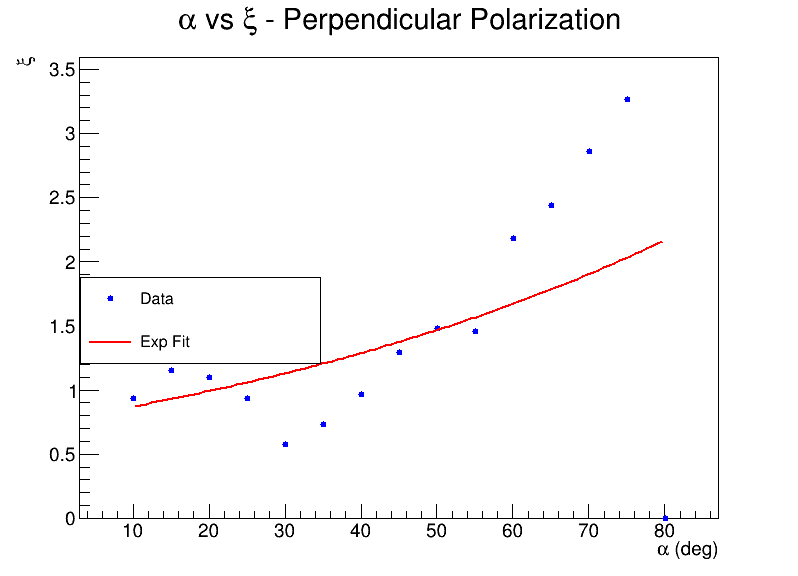
\includegraphics[width=\linewidth]{../plots/perpendicular_plot.png}
    \caption{$\xi_{\perp}$ vs $\alpha$ - Perpendicular Polarization. Data points (blue) show increasing reflected intensity with angle. The red line represents an exponential fit.}
    \label{fig:perpendicular}
\end{figure}
\begin{figure}[H]
    \centering
    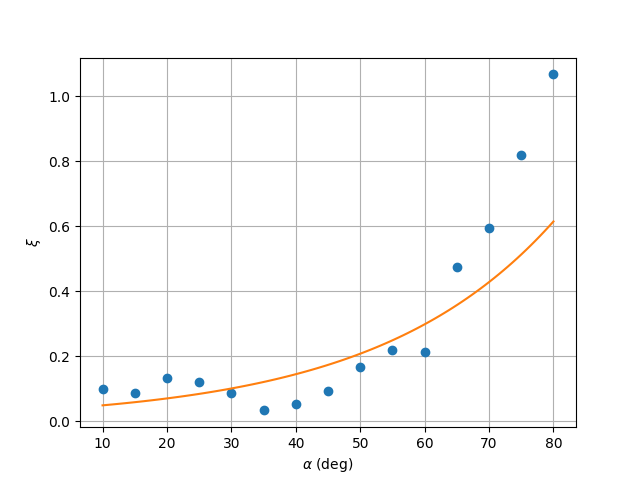
\includegraphics[width=\linewidth]{../plots/exponential_fit.png}
    \caption{Exponential fit for $\xi_{\perp}$ vs $\alpha$ - Perpendicular Polarization. The orange curve represents the fitted exponential model, closely matching the experimental data points (blue).}
    \label{fig:exponential_fit}
\end{figure}
Figure \ref{fig:parallel} shows the reflected intensity for parallel polarized light ($\xi_{\parallel}$) versus the angle of incidence ($\alpha$). The intensity first decreases, reaches a minimum value at an intermediate angle, and then increases again at larger angles. This behavior is characteristic of $R_p$ according to Fresnel's equations. The minimum intensity corresponds to Brewster's angle ($\theta_B$). A polynomial fit (Poly4) was applied in the original analysis.
\begin{figure}[H]
    \centering
    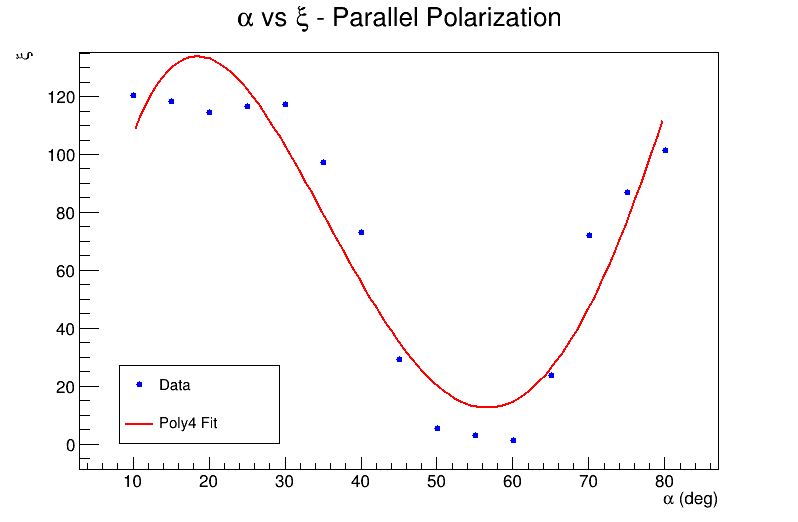
\includegraphics[width=\linewidth]{../plots/parallel_plot.png}
    \caption{$\xi_{\parallel}$ vs $\alpha$ - Parallel Polarization. Data points (blue) show a minimum intensity around $\alpha \approx \SI{55}{\degree}$. The red line represents a polynomial (degree 4) fit.}
    \label{fig:parallel}
\end{figure}
\begin{figure}[H]
    \centering
    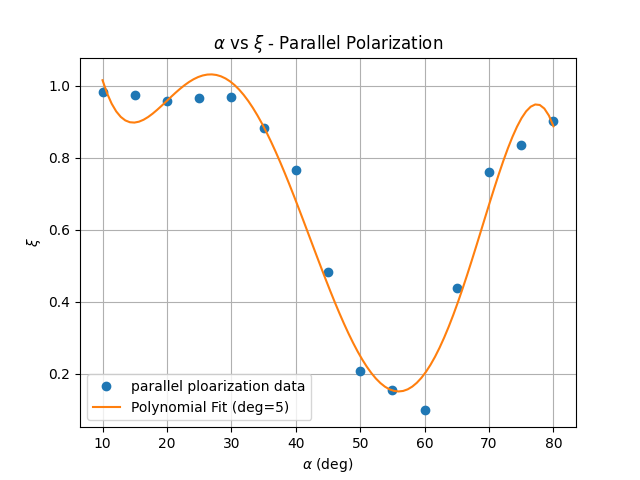
\includegraphics[width=\linewidth]{../plots/polynomial_fit.png}
    \caption{Polynomial fit for $\xi_{\parallel}$ vs $\alpha$ - Parallel Polarization. The orange curve represents the fitted polynomial model (degree 3), closely matching the experimental data points (blue).}
    \label{fig:polynomial_fit}
\end{figure}
\section{Discussion}
The experimental results align well with the theoretical predictions based on Fresnel's equations.

For perpendicular (s-) polarization, the reflected intensity $\xi_{\perp}$ increases monotonically with the angle of incidence $\alpha$, as shown in Figure \ref{fig:exponential_fit}. The exponential fit applied to the data closely matches the experimental points, confirming the expected behavior of $R_s$, which increases from a value at normal incidence ($\alpha=0$) towards 1 at grazing incidence ($\alpha=\SI{90}{\degree}$). This trend is consistent with Fresnel's equations for s-polarized light.

For parallel (p-) polarization, the reflected intensity $\xi_{\parallel}$ exhibits the characteristic dip associated with Brewster's angle, as shown in Figure \ref{fig:polynomial_fit}. The polynomial fit (degree 3) highlights a minimum intensity near $\alpha \approx \SI{55}{\degree}$. The minimum value is approximately $\xi_{\parallel} \approx 1.2$ (arbitrary units) at $\alpha = \SI{60}{\degree}$, but visually inspecting the data points suggests the minimum might occur between $\SI{50}{\degree}$ and $\SI{60}{\degree}$. The polynomial fit provides a smooth representation of the data, suggesting Brewster's angle is approximately $\theta_B \approx \SI{55 \pm 5}{\degree}$.

Ideally, the intensity at Brewster's angle should be zero for p-polarized light. The observed non-zero minimum ($\xi_{\parallel} \approx 1.2$) could be attributed to several factors:
\begin{itemize}
    \item The incident light might not have been perfectly linearly polarized.
    \item The polarization axis might not have been perfectly aligned parallel to the plane of incidence.
    \item The light source might not have been perfectly monochromatic.
    \item Scattering from surface imperfections.
    \item Detector noise or offset.
    \item Finite angular resolution of the setup.
\end{itemize}

Assuming Brewster's angle is approximately $\theta_B \approx \SI{55}{\degree}$, and the incident medium is air ($n_1 \approx 1$), we can estimate the refractive index ($n_2$) of the dielectric material using Equation \ref{eq:brewster}:
\begin{equation}
    n_2 = \tan(\theta_B) \approx \tan(\SI{55}{\degree}) \approx 1.43
\end{equation}
If we take the minimum closer to $\SI{58}{\degree}$ (based on the fit's appearance near the minimum), $n_2 \approx \tan(\SI{58}{\degree}) \approx 1.60$. A value around 1.5 is typical for glass. The uncertainty in determining the exact minimum from the discrete data points and the non-zero minimum intensity limits the precision of this estimation.

\section{Conclusion}
This experiment successfully investigated the reflection of linearly polarized light from a dielectric surface as a function of the angle of incidence. The measured reflected intensities for perpendicular ($\xi_{\perp}$) and parallel ($\xi_{\parallel}$) polarizations generally followed the trends predicted by Fresnel's equations. The intensity for perpendicular polarization increased with the angle of incidence. The intensity for parallel polarization showed a distinct minimum, identifying Brewster's angle.

From the data, Brewster's angle for the sample material was estimated to be $\theta_B \approx \SI{55 \pm 5}{\degree}$. This corresponds to an estimated refractive index of the material $n_2 \approx 1.43 - 1.73$ (using $\SI{55}{\degree}$ to $\SI{60}{\degree}$), consistent with common materials like glass. The non-zero minimum intensity observed for parallel polarization suggests minor experimental imperfections or limitations. Overall, the experiment provides a clear demonstration of polarization-dependent reflection and the phenomenon of Brewster's angle.

\section{Additional Resources}
For detailed information, including the Lab Manual, source code, and related experiments, visit the GitHub repository provided below or scan the QR code in Fig.~\ref{fig:qr_code}.

\begin{figure}[H]
    \centering
    \begin{minipage}{0.15\textwidth}
        \centering
        \qrcode[height=2cm]{https://github.com/ibeuler/LAB-Reports}
    \end{minipage}%
    \begin{minipage}{0.2\textwidth}
        \raggedright
        \caption{Access the GitHub repository for the lab manual, source code, and related experiments: \href{https://github.com/ibeuler/LAB-Reports}{\url{https://github.com/ibeuler/LAB-Reports}}.}
        \label{fig:qr_code}
    \end{minipage}
\end{figure}

\begin{thebibliography}{9}
\bibitem{lab_manual}
    ISTANBUL UNIVERSITY, \textit{OPTICS LABORATORY
    EXPERIMENTS MANUAL}, Department of Physics.

\bibitem{github}
    \textit{Source code and additional experiments are available in the GitHub repository.} \url{https://github.com/ibeuler/LAB-Reports}
\end{thebibliography}
\end{document}